\section{Where Diffusion Wins, and Where It Doesn't}
\label{sec:fair}

\subsection{The surviving advantage, and what it is measured against}

At its natural output length, AR-1.5B completes a record in 665.7\,ms at 138
output tokens (unforced, \texttt{min\_tokens}\,$=$\,0). At forced output
$L \geq 512$ tokens, the diffusion model is faster at matched quality. The
advantage grows with output length because the AR model pays per token while
the diffusion model pays per canvas.

\begin{table}[h]
\centering
\caption{Latency at matched quality (AR-1.5B vs DG-26B-A4B, batch-1). AR
cells are \emph{forced} (\texttt{min\_tokens}\,$=$\,$L$); unforced AR-1.5B
completes in 665.7\,ms at 138 tokens.}
\label{tab:niche}
\begin{tabular}{@{}lrrrr@{}}
\toprule
$L_{\mathrm{out}}$ & AR-1.5B forced (ms) & AR-1.5B unforced & DG (ms) & DG advantage \\
\midrule
138 (natural) & --- & 665.7 & \dgTwoFive{} & $1.8\times$ \\
256  & \arOneFiveTwoFive{} & --- & \dgTwoFive{}   & $2.7\times$ \\
512  & \arOneFiveFiveOne{} & --- & \dgFiveOne{}   & $4.0\times$ \\
1024 & \arOneFiveTenTwoFour{} & --- & \dgTenTwoFour{} & $5.4\times$ \\
\bottomrule
\end{tabular}
\end{table}

The diffusion model is faster even unforced: at AR-1.5B's natural output
length of 138 tokens, DG completes in \dgTwoFive\,ms against AR's 665.7\,ms
--- a $1.8\times$ advantage. Forcing the AR arm to emit $L{=}1024$ tokens
inflates that to $5.4\times$, because first-object-wins parsing
(\S\ref{app:defects}, defect 3) discards the rambled continuation past the
first JSON object. At $L{=}1024$ the AR arm is charged
\arOneFiveTenTwoFour\,ms for output the scorer deletes. The
$4.0$--$5.4\times$ advantage therefore measures the cost of
\texttt{min\_tokens}, not the cost of autoregression --- it is an upper bound
on AR cost, not a measurement of it. The real advantage is $1.8\times$, and
a $1.8\times$ gap on a model \footprintRatio$\times$ larger is not a
deployment argument.

\begin{figure}[t]
\centering
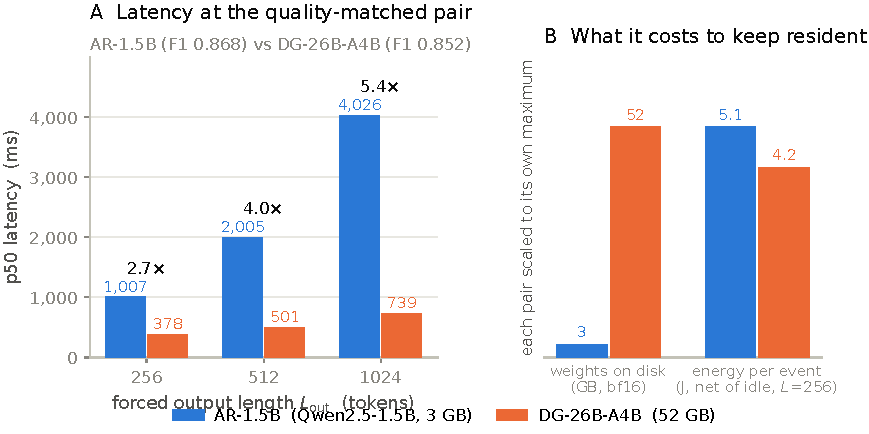
\includegraphics[width=\linewidth]{figures/fig9_deployment.pdf}
\caption{The quality-matched deployment pair. \textbf{A:} at forced output
lengths the diffusion model's advantage is real and grows, because the AR
model rambles well past its natural length ($\sim$\naturalLar\ tokens) and
vLLM still processes every forced token. \textbf{B:} the standing cost of
keeping each model resident.}
\label{fig:deploy}
\end{figure}

The diffusion model also degrades gracefully under deadline pressure: it
returns a complete canvas at lower quality, while the AR model returns a
truncated record that fails schema validation. At a p99 budget of 400\,ms,
dropping $K$ from 8 to 4 meets it at \kFourPninetynine\,ms p99 with F1 falling
from \kEightFone\ to \kFourFone.

\subsection{Why the advantage usually doesn't survive}

Three factors close the niche:

\paragraph{Footprint.} The quality-matched AR model (Qwen2.5-1.5B, F1
\arOneFiveFnine) is \arOneFiveWeights\,GB; the diffusion model is
\dgWeights\,GB --- a \footprintRatio$\times$ difference.

\paragraph{Batching.} Continuous batching converts arrival concurrency into
throughput at \arBatchLo--\arBatchHi$\times$ for AR against
$\leq$\dgBatchVllmHi$\times$ for diffusion. Both diffusion measurements are
engine-bounded (vLLM caps the batch at 8; dInfer runs cache-less), so the
true ceiling is unknown but lies at or above \dgBatchVllmHi$\times$. Even so,
the gap is more than an order of magnitude (Appendix~\ref{app:batching}).

\paragraph{Input length.} The diffusion prefill slope is
\inputSlopeRatio$\times$ steeper, because each denoising step re-attends the
full prompt. At longer inputs the base rises and $L^{*}$ moves upward.

\begin{figure}[t]
\centering
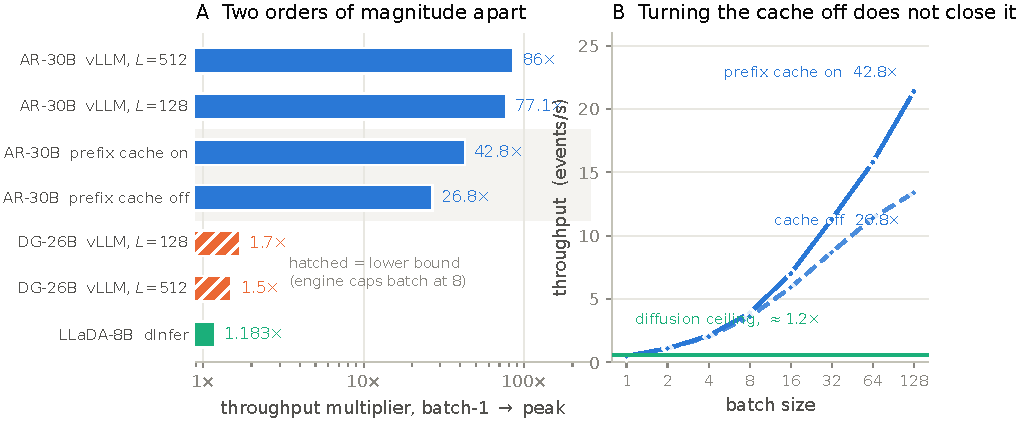
\includegraphics[width=\linewidth]{figures/fig6_batching.pdf}
\caption{Batch-1 to peak throughput multipliers. The split runs along
architecture, not runtime: two diffusion models on two different engines sit
at $\leq$\dgBatchVllmHi$\times$, while the AR model on vLLM ranges from
\cacheOffMult$\times$ to \arBatchHi$\times$.}
\label{fig:batching}
\end{figure}

\subsection{The five conditions}

The diffusion model is the right choice only when all five hold:
\begin{enumerate}[nosep]
  \item Output length $\geq 512$ tokens, forced (untested at naturally-long
    output; see \S\ref{sec:threats}).
  \item Batch-1 by requirement (tenant isolation, interactivity).
  \item Completeness is validated against a schema.
  \item The quality floor exceeds what the AR model delivers.
  \item A \dgWeights\,GB resident footprint is acceptable.
\end{enumerate}
